\section{Standardisierung der Schnittstellennavigation}

Wie insbesondere bei ergonomischen Inspektionen und Benutzertests beobachtet wurde, kann die Schnittstelle für den Benutzer manchmal verwirrend sein, da er oft den roten Faden der Schnittstelle zu verlieren scheint.
Dennoch gibt es zahlreiche Regeln und Standards für Schnittstellen, die es dem Benutzer erleichtern, sich in einer komplexen Schnittstelle zurechtzufinden.
In diesem Abschnitt werden einige Strategien vorgestellt, die in der endgültigen Schnittstelle implementiert werden.

\subsection{Lokalisierung von Seiten}

Wenn ein Benutzer zwischen verschiedenen Seiten einer Webanwendung navigiert, muss er sehr schnell erkennen können, auf welcher Seite er sich befindet.
Wenn er keine normierte Referenz auf der Schnittstelle hat, kann es ihn Zeit und kognitive Belastung kosten, die Schnittstelle zu identifizieren, auf der er sich befindet, und die Verbindung nachzuvollziehen, die sie mit den anderen Schnittstellen der Anwendung hat.
Dies kann passieren, wenn sie viel zurückgehen, um eine zuvor geöffnete Seite erneut zu besuchen, oder wenn sie von einer Seite zu einer anderen weitergeleitet werden.
Schlimmer noch, wenn der Nutzer auf eine neue Seite gelangt, die er nicht kennt, muss er die Schnittstelle untersuchen, um zu versuchen, den Kontext der Seite zu erfassen, was eine unnötige Anstrengung erfordert.
Die beiden folgenden Beispielseiten haben zum Beispiel keine klaren Elemente, die es dem Nutzer ermöglichen, schnell zu erkennen, auf welcher Seite er sich befindet.

\begin{figure}[H]
  \centering
  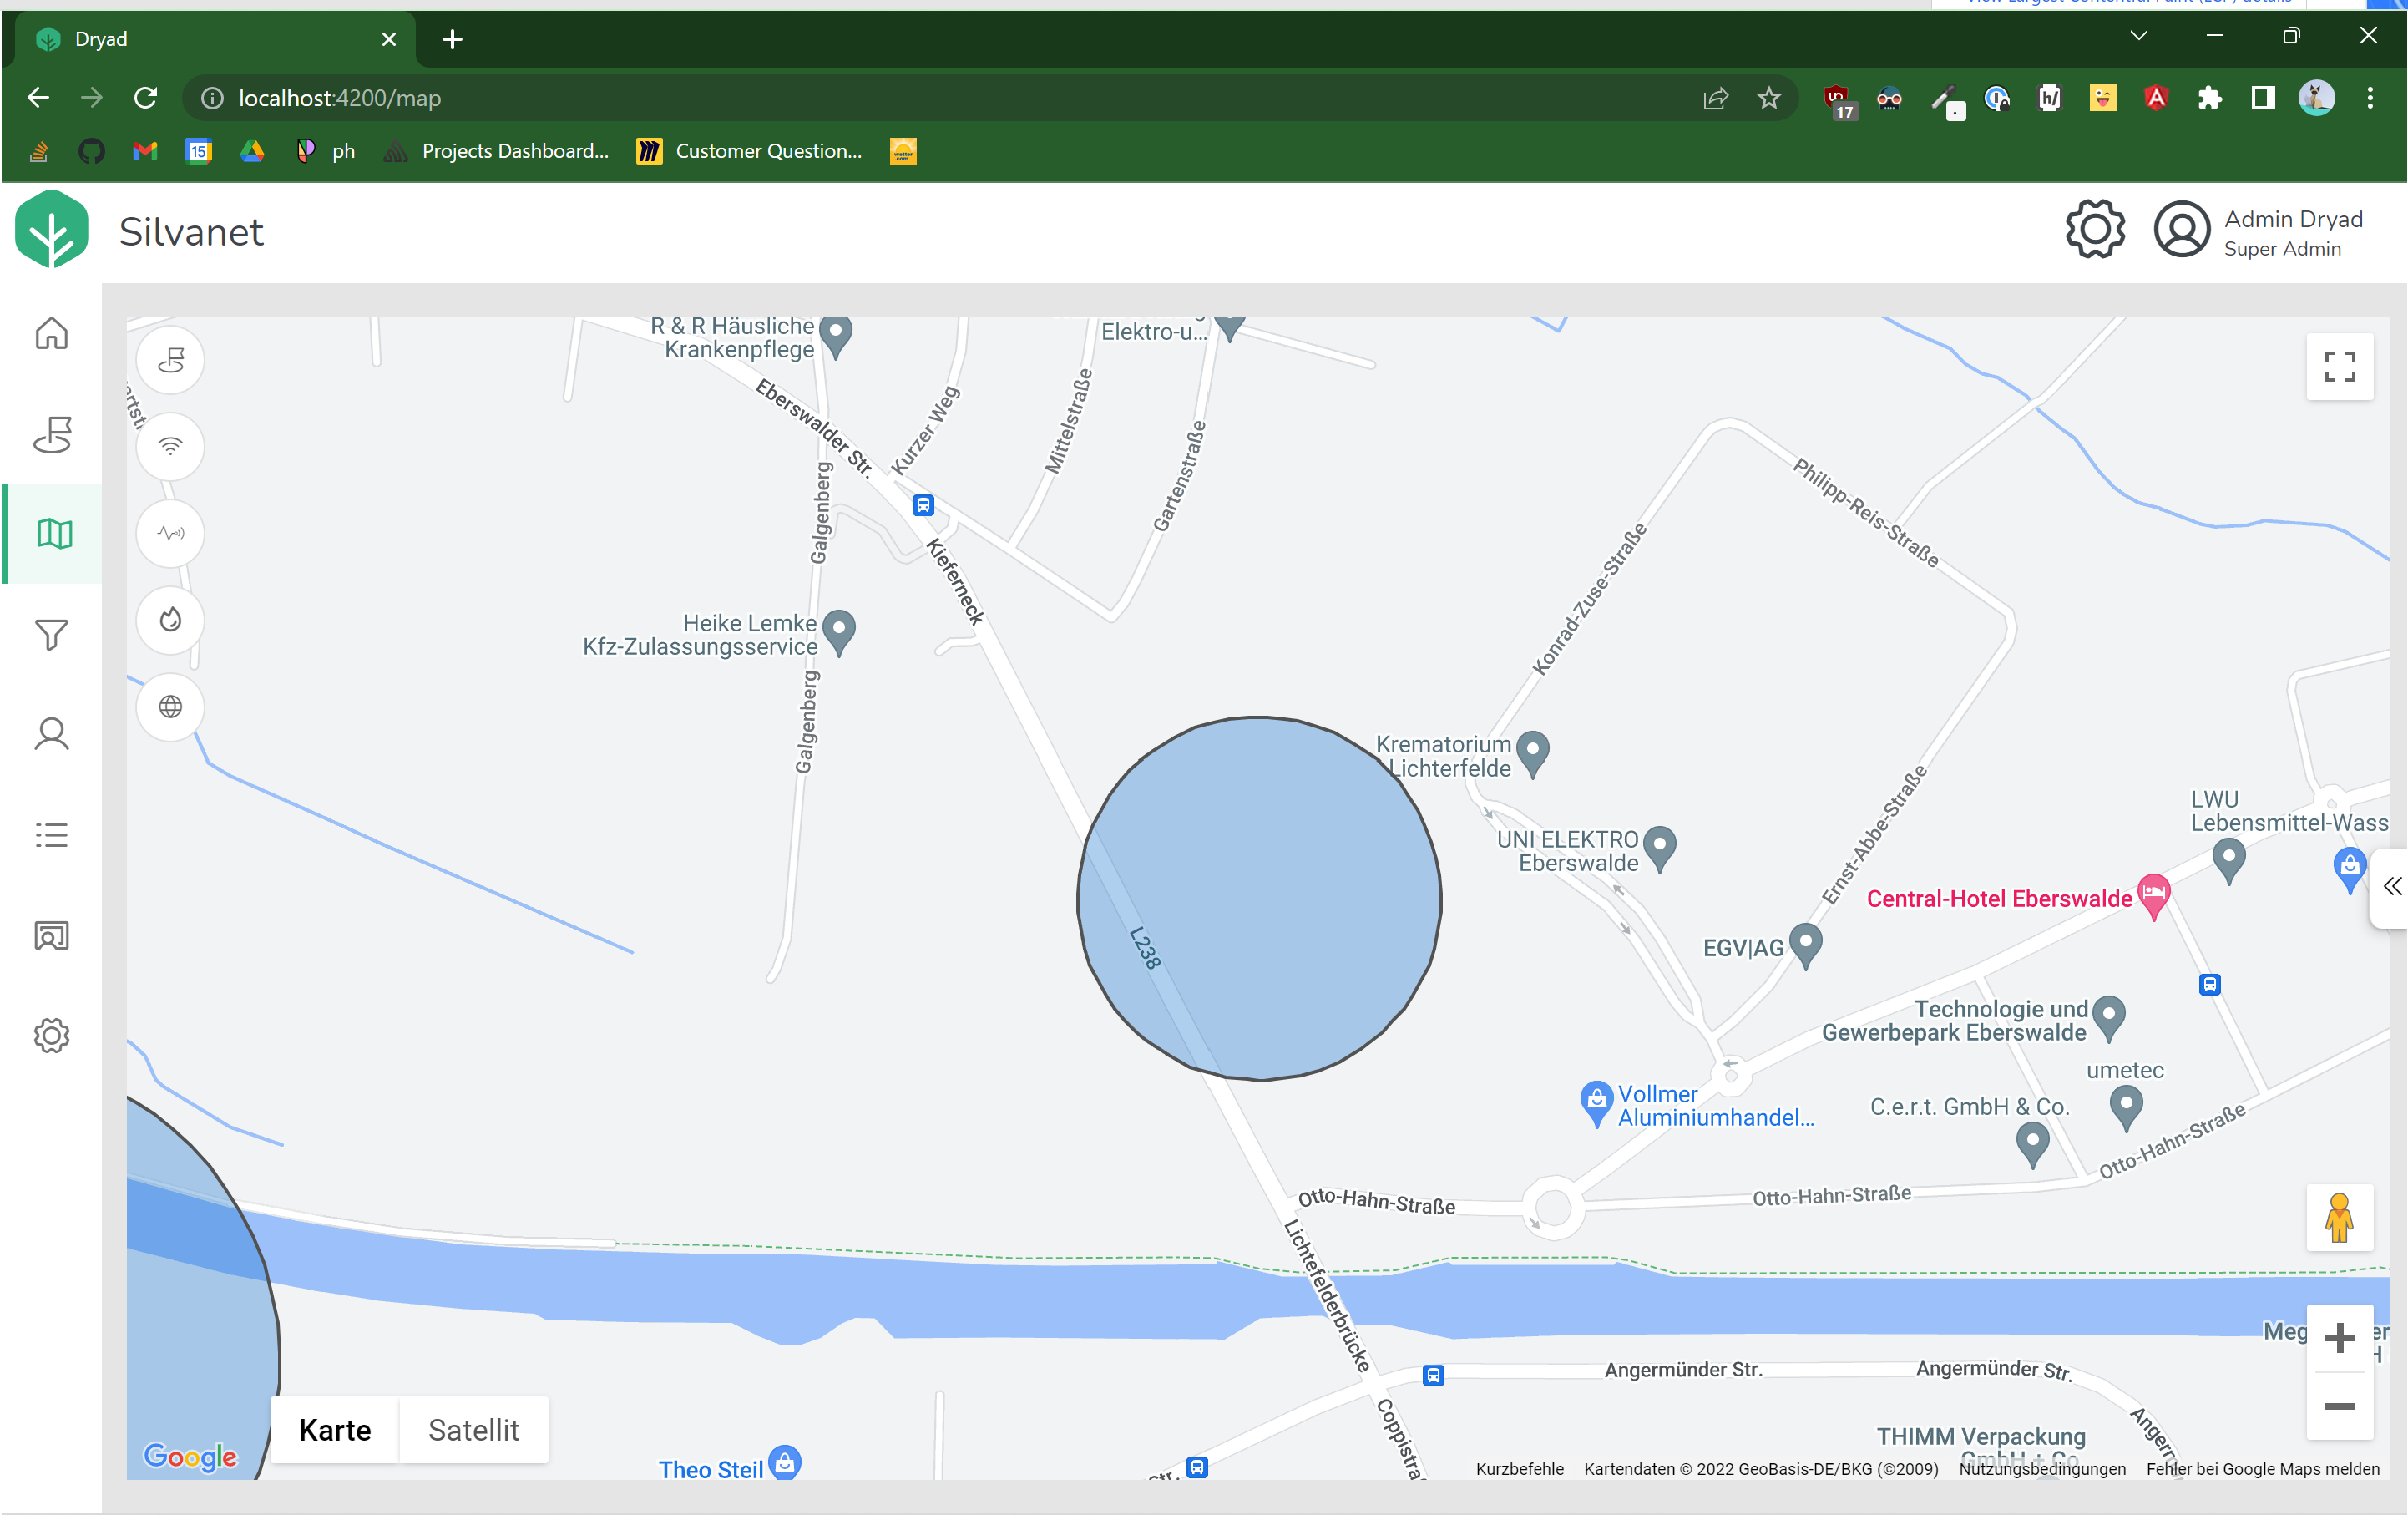
\includegraphics[width=\textwidth]{app_page_map_old}
  \caption{Seite der Schnittstelle mit einer interaktiven Karte der verschiedenen \textit{Sites}}
  \label{fig:app_page_map_old}
\end{figure}
\begin{figure}[H]
  \centering
  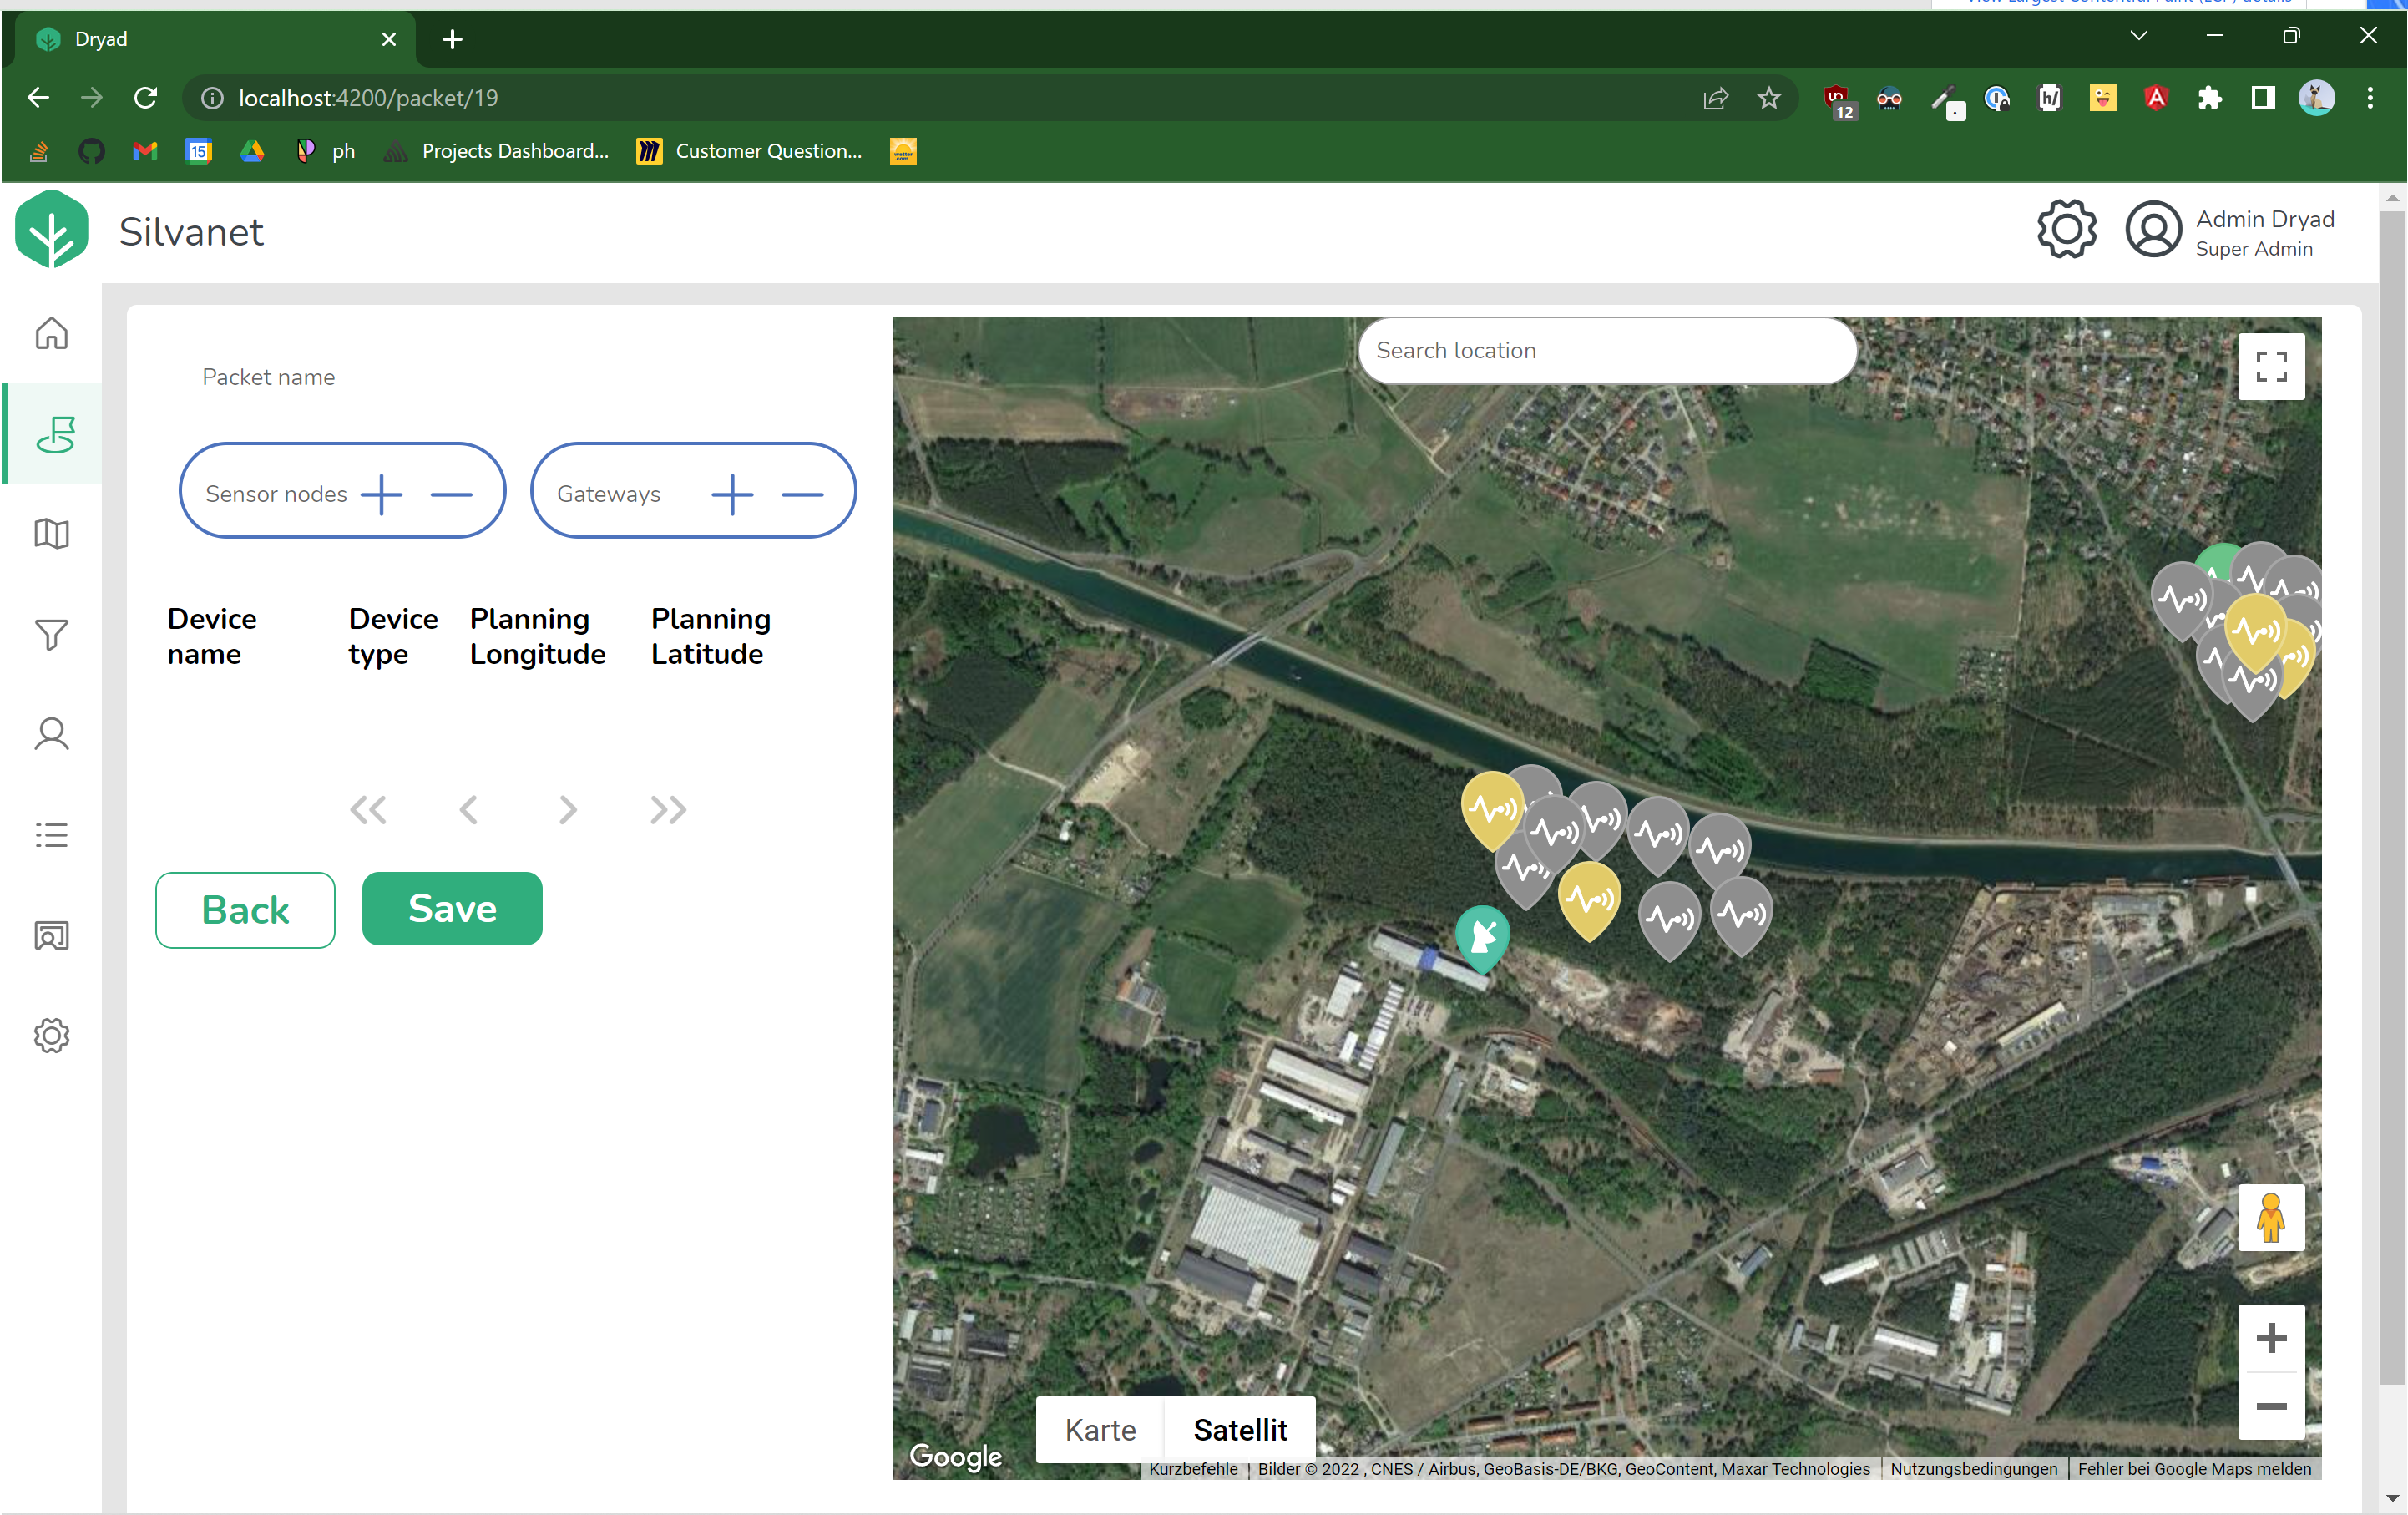
\includegraphics[width=\textwidth]{app_page_planning_old}
  \caption{Seite der Schnittstelle, mit der Sie den Einsatz von Sensoren an einem \textit{Sites} planen können.}
  \label{fig:app_page_planning_old}
\end{figure}

Auf diese Weise ist es für einen Nutzer nicht möglich, zu definieren, auf welcher Seite er sich befindet.
Es gibt jedoch viele standardisierte Strategien, die ein entspanntes Surfen ermöglichen.
Die erste, die sogar ein Muss für die Zugänglichkeit einer Schnittstelle ist, ist das Vorhandensein eines aussagekräftigen Seitentitels.
Dieser Seitentitel wird in \ac{HTML} im Header der Seitenstruktur deklariert und ermöglicht es, einen benutzerdefinierten String in der Titelleiste des Browsers, im Seitenfenster oder auch im Verlauf des Browsers anzuzeigen.
Anhand eines aussagekräftigen Titels kann ein Benutzer leicht erkennen, welche Webseite er gerade benutzt und wann sich die Webseite geändert hat.
Der Titel kann zur Identifizierung der Webseite verwendet werden, ohne dass die Benutzer den Inhalt der Seite lesen oder interpretieren müssen.
Die Benutzer können den gewünschten Inhalt schneller finden, wenn genaue, beschreibende Titel in Sitemaps oder Listen von Suchergebnissen erscheinen.

So empfehlen die Zugänglichkeitsstandards der \ac{WCAG}\cite{wcag}, dass der Titel einer Seite in der Lage ist:

\begin{itemize}
  \item Das Thema der Webseite identifizieren
  \item Sinn machen, wenn sie ohne Kontext gelesen werden, z. B. in einer Website-Karte oder einer Liste von Suchergebnissen
  \item Kurz sein
  \item Angabe der Website oder einer anderen Ressource, zu der die Webseite gehört
\end{itemize}

Eine Struktur, die von der großen Mehrheit der Web-Schnittstellen verwendet wird, kann durch die folgende Notation dargestellt werden\\
\lstinline{<Eindeutiger Titel der Seite> <Trenner> <Titel der Anwendung>}.

Im Fall der Silvanet-Anwendung von Dryad wurden die folgenden Standards festgelegt:

\begin{itemize}
  \item \textbf{<Titel der Anwendung>}: Dryad
  \item \textbf{<Trenner>}: •
\end{itemize}

Die Anwendung muss also in der Lage sein, für jede Seite einen Titel vorzuschlagen, der diesem Standard entspricht.
Jetzt müssen Sie dem Nutzer auch noch einen Seitentitel anbieten, der für die Seite selbst relevant ist.
Wie man in \ref{fig:app_page_map_old} und \ref{fig:app_page_planning_old} sehen kann, bleibt der Haupttitel der Seite, der dem \lstinline{h1}-Tag in \ac{HTML} entspricht, nämlich konstant das gleiche Wort \textit{Silvanet}.

Die Schnittstelle sollte an dieser Stelle auch einen Begriff verwenden, der den Kontext der Seite beschreibt, so dass er den Seitentitel widerspiegelt.
Hier ist ein Beispiel für eine Kombination von Seitentiteln mit einem relevanten, standardisierten und kontextbezogenen Hauptseitentitel.

\begin{table}[H]
  \begin{tabular}{p{0.5\linewidth} |p{0.5\linewidth}}
    Seitentiteln                   & Hauptseitentitel \\ \hline\hline

    \textit{Sites • Dryad}         & Sites Management \\\hline
    \textit{User Settings • Dryad} & User Settings    \\\hline
    \textit{Dashboard • Dryad}     & Dashboard
    \\\hline
  \end{tabular}
  \caption{Beispiel für eine Kombination von Seitentiteln mit einem Hauptseitentitel}
\end{table}

\subsection{Übersichtliches Navigationssystem}

Die Navigation des Nutzers sollte so einfach wie möglich gestaltet werden, damit es keine Ambiguität gibt, die es dem Nutzer erlaubt, die Oberfläche selbst zu erkunden.
Die ergonomische Inspektion \ref{appendix:ergonomic-inspection} zeigt jedoch einen großen Usability-Fehler in der Seitenleiste der Anwendung, die als Navigationsmenü fungiert.
Es besteht nur aus Icons, die, wie im Punkt \ref{sec:guidance} erläutert, sehr subjektiv und hängen von der Kultur des Nutzers ab.
Es ist daher notwendig, jedem Icon ein Textlabel hinzuzufügen, um die Verständlichkeit der Icons im Menü zu standardisieren.
Dies nimmt jedoch Platz auf der Benutzeroberfläche in Anspruch, da der Benutzer diese Aktion schnell beherrschen und verstehen muss.
Nach mehreren Besuchen auf der Benutzeroberfläche wird der Benutzer natürlich eine Verbindung zwischen den Icons und dem Label herstellen.
So ist es sinnvoll, dass der Nutzer jederzeit entscheiden kann, ob er die Textkennzeichnungen ausblenden oder anzeigen möchte.
In dieser Situation kann ein Kollaps-System verwendet werden.

\begin{table}[H]
  \begin{tabular}{p{0.5\linewidth} |p{0.5\linewidth}}
    Menü mit Textlabels & Reduziertes Menü nur mit Icons \\ \hline\hline

    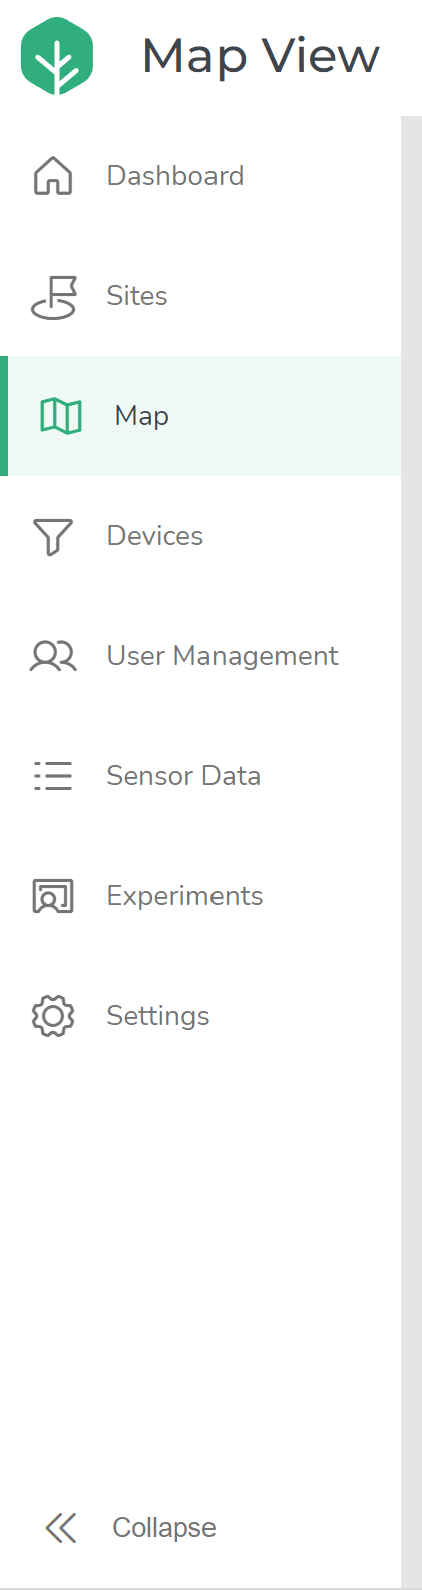
\includegraphics[height=12cm]{app_sidebar_open}
                        &
    
\includegraphics[height=12cm]{app_sidebar_collapsed}
  \end{tabular}
  \caption{Menü in der Sidebar, das ein Kollaps-Design implementiert}
\end{table}
